\newcommand{\AND}{\texttt{AND}\xspace}

\section{Multiplier}


\subsection{Wallace Tree Multiplier}

For this project it was decided the most appropriate multiplier scheme would be the Wallace Tree Multiplier. The most important reason for this choice is due to its great performance although at the cost of gates and area.

The Wallace tree is a regular hardware structure to multiply two operands.
It was invented by Chris Wallace in 1964.

The algorithm can be divided in three major steps:
\begin{enumerate}
\item The initial \AND operation between all combinations of bits of each operand. The weights must be adjusted according to the location of the operands, just like in the classical pen-and-paper algorithm. The resulting tree, using dot notation, is shown in figure~\ref{fig:wallace_tree}.

\begin{figure}[H]
\centering
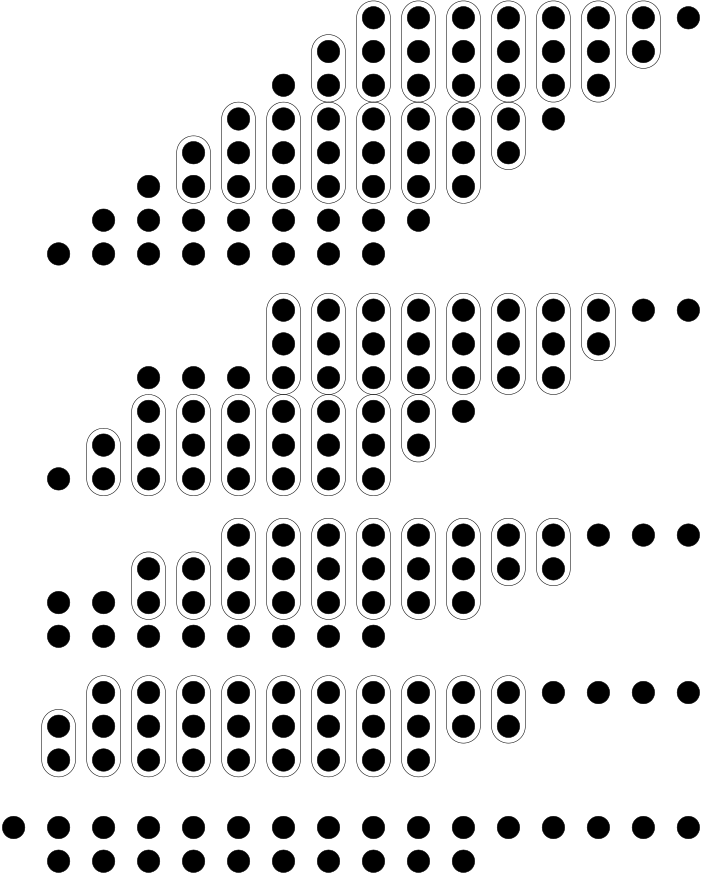
\includegraphics[width=0.45\textwidth,height=0.2\textheight,keepaspectratio]{Wallace_tree.png}
\caption{Resulting tree after executing step 1 for and 8 bit by 8 bit multiplication.}
\label{fig:wallace_tree}
\end{figure}

\item Thereafter the tree must be reduced through the use of half adder and full adders. These will convert each two or three ``dots'', respectively, into one and a carry out for the following column. This step shall be iterated sufficient times until only only two numbers remain.

\item Finally, the two remaining numbers can be summed with a conventional adder. The width of the result should be equal to the sum of the widths of the original operators. For example for a 32 bit times 32 bit operation, the result shall be 64 bits wide. 
\end{enumerate}  

For our particular implementation the aforementioned description was modified to accommodate signed numbers through the use of the modified Baugh-Wooley algorithm. The details of this alteration will be explained in section~\ref{sec:implementation}.

\subsection{Advantages and Disadvantages}

The main advantages of this scheme is the speed obtained and regular mapping in hardware. The structure of the tree is consistent throughout the several steps. On the other this design is costly in the amount of gates used and there is some waste of area. This is particular noticeable on the extremes of each line of the tree, as shown in figure~\ref{fig:paper_wastedarea}. \Cite{betterwallace} details possible improvements that can be accomplished in this regard to improve the area cost of the Wallace multiplier. The main idea is to split the tree into two overlapping trees, hence saving area. Thereafter the additions take place in opposite directions. 
However due to lack of time it was not possible to implement the proposed ideas.

\begin{figure}[H]
\centering

\subfloat[Detail of Wallace Tree from~cite{betterwallace}. It is clearly visible a significant percentage of unused area.]{\label{fig:paper_wastedarea}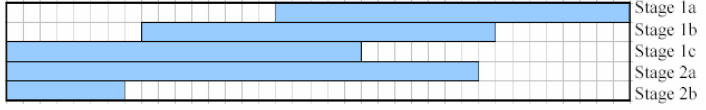
\includegraphics[width=0.45\textwidth,height=0.2\textheight,keepaspectratio]{paper_wastedarea.png}}\qquad
\subfloat[Modified Wallace Tree from~cite{betterwallace}. The image reflects the better area utilization based on the algorithm present in the paper.]{\label{fig:paper_improvedarea}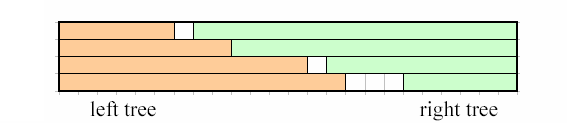
\includegraphics[width=0.45\textwidth,height=0.2\textheight,keepaspectratio]{paper_improvedarea.png}}
\caption{}
\label{fig:paper}
\end{figure}


\subsection{Implementation and Simulation Results}
\label{sec:implementation}